
\subsection{Definition}

% \begin{defn}
% Let $(M,\xi)$ be a contact manifold. A \wddef{Legendrian knot} $L$ in $(M,\xi)$ is
% an embedding $\gamma: S^1 \to M$, such that $L = \gamma(S^1)$ and 
% \[ \left. \dif{\gamma}{t} \right|_{t'} \subset \xi_{\gamma(t')}. \] 
% \end{defn}

\begin{defn}
Let $(M,\xi)$ be a contact manifold. A \wddef{Legendrian knot} $L \subset M$ is
an embedding of $S^1$, such that 
\begin{equation}
\label{eq:l_knot_eq}
T_x L = \xi_x, \quad \forall x\in L. 
\end{equation}
\end{defn}

For the rest of this paper we will assume $(M,\xi) = (\R^3,\xi_{std})$. Most of
the discussions and result generalize to general contact manifolds. But for
simplicity we will stick with this particular case. This allows us to work in
terms of the projections onto the coordinate planes, which will simplify some of
the arguments significantly. In particular the proofs found in chapter
\pref{chap:proofs}, will naturally simplify to a combinatorial argument.

\subsection{Projections}

For this section it will convenient to have a parametrization for $L$. Let
\[ \gamma : S^1 \to L; \: t \mapsto (x(t), y(t),z(t)), \] 
be a $C^1$ (ones continuously differentiable) parametrization of $L$. Then we 
can be written equation \pref{eq:l_knot_eq},
\[ \gamma'(t) \subset \xi_{\gamma(t)}, \quad \forall t\in S^1, \] 
or equivalently, since $\xi = \xi_{std} = \ker{\d z - y\d x}$, 
\begin{equation}
\label{eq:std_l_knot_eq}
z'(t) - y(t) x'(t) = 0.
\end{equation}

\begin{defn}
\wddef{Front projection} is the map
\[ \Pi : \R^3 \to \R^2; \: (x,y,z) \mapsto (x,z), \]
\end{defn}

Let $\phi_\Pi = \Pi \circ \gamma$.  By equation \pref{eq:std_l_knot_eq}, $z'(t)
= y(t) x'(t)$, so if $x'(t) = 0$, $z'(t) = 0$. Therefore $\Pi(L)$ can not have
any vertical tangents \big(ie.  $\phi_\Pi'(t) \notin \spann\qty{\dd{z}}
\setminus\{0\}$ for all $t$. \big) Also $(\phi_\Pi)'(0) = 0$, whenever $x'(t) =
0$, so $\phi_\Pi$ is on not an immersion. On the other hand, away from $x'(t) =
0$ (ie. $t \in I \setminus x'^{-1}(0)$), $\phi_\Pi$ is an immersion.  If $x'(t)
\ne 0$, by equation \pref{eq:std_l_knot_eq}, we may recover $y(t)$ from the
projection
\[ y(t) = \frac{z'(t)}{x'(t)}. \]

A point in $\Pi(L)$ where $x'(t) = 0$ we will call a "cusp point". Here the
tangent of $L$ is parallel with the $y$-axis. See figure \pref{fig:cusp_point}.

\begin{figure}
\centering
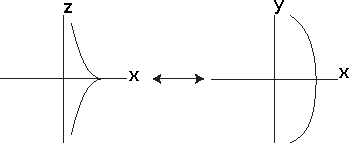
\includegraphics[width=.4\textwidth]{figs/cusp_point.pdf}
\caption{Front and Lagrangian projection of a part of a Legendrian knot where
$x'(t) = 0$ (ie. a cusp point, in the front projection.)}
\label{fig:cusp_point}
\end{figure}

\begin{lemma}
A diagram $D \subset \R^2$, is the Front projection of a Legendrian knot
if and only if:
\begin{enumerate}
\item
There are no vertical tangents.
\item 
$D$ is an immersion away from a finite collection of cusp, points.
\item 
At each crossing the slope of the overcrossing is less then the slope of the
undercrossing.
\end{enumerate}
\end{lemma}

\begin{exmp}
In figure \pref{fig:front_knots} we can see the front projection of a Legendrian
realization of the unkont, left and right handed trefoil knot and the figure of
eight knot.
\end{exmp}

\begin{figure}[h]
\centering
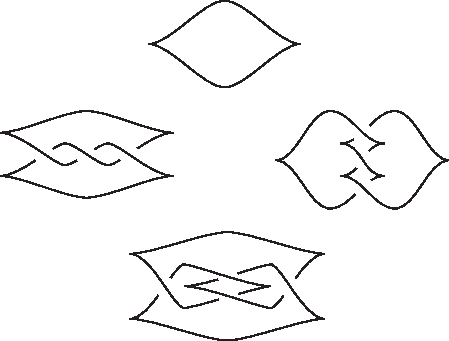
\includegraphics[width=.4\textwidth]{figs/front_knots.pdf}
\caption{Front projection of Legendrian realization of the unknot, left and
right handed trefoil knots and the figure of eight knot.}
\label{fig:front_knots}
\end{figure}

\begin{defn}
The \wddef{Lagrangian projection} of $L$ is the map
\[ \pi : \R^3 \to \R^2; \: (x,y,z) \to (x, y), \]
\end{defn}

Let $\phi_\pi = \pi \circ \gamma$. In contrast with the front projection,
$\phi_\Pi$ is always an immersion, since by equation \pref{eq:std_l_knot_eq}, if
$x'(t) = 0$ also $z'(t) = 0$ and thus $y'(t) \ne 0$, as $\phi$ is an immersion.

By integrating equation \pref{eq:std_l_knot_eq}, we have 
\[ z(t) = z_0 + \int_0^t y(t') x'(t') \d t',  \]
( Here we consider $t \in [0,2\pi)$ ) so we may recover the z-component of $L$ from the projection up to an overall
factor $z_0$. Note that for $L$ to be closed we require $z(2\pi) = z_0$, so 
\begin{equation}
\label{eq:lagrangian_pr_eq}
\int_S^1 y(t) x'(t) \d t = 0.
\end{equation}

\begin{lemma}
A diagram $D \in \R^2$ is the Lagrangian projection of a Legendrian knot if and
only if
\begin{enumerate}
\item $D$ is an immersion.
\item 
$\int_S^1 y(t) x'(t) \d t = 0$, where $(x,y): S^1 \to \R^2$ is a
parameterization of $D$.
\item 
$\int_{t_1}^{t_2} y(t) x'(t) \d t = 0$, if $(x(t_1),y(t_1)) = (x(t_2),y(t_2))$.
\end{enumerate}
\end{lemma}

This projection will be the more interesting for us. Though the constraints (ie.
\pref{eq:lagrangian_pr_eq}), given by the Legendrian condition \pref{eq:l_knot_eq}, is a little harder to work with. 

\section{Reidemeister moves}

Like in the case of topological knots, there are also Legendrian Reidemeier
moves for these projections, see figure \pref{fig:reid_move_top}

\begin{figure}
\begin{minipage}[c]{.5\textwidth}
\centering
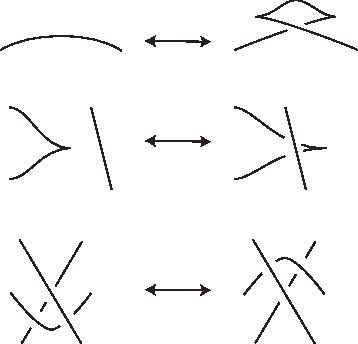
\includegraphics[width=.8\textwidth]{figs/reid_moves_front.pdf}
\caption{Legendrian Reidemeister moves in front projection.}
\label{fig:reid_move_top}
\end{minipage}
\begin{minipage}[c]{.5\textwidth}
\centering
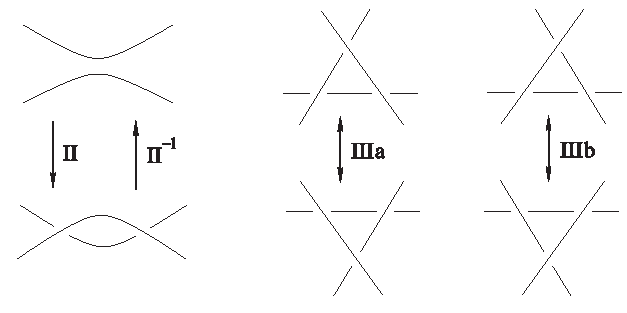
\includegraphics[width=.8\textwidth]{figs/reid_moves.pdf}
\caption{Legendrian Reidemeister moves in Lagrangian projection.}
\label{fig:reid_move_top}
\end{minipage}
\end{figure}

% \subsection{The existence of Legendrian knots of any top know}
